\section{Giới thiệu dự án}
Việt Food là một ứng dụng web fullstack với kiến trúc client-server nhằm cung cấp nền tảng đặt món ăn Việt Nam trực tuyến. Ứng dụng được phát triển với mục đích tạo ra trải nghiệm người dùng hiện đại, thân thiện, đồng thời đảm bảo hiệu suất cao và khả năng mở rộng. Với giao diện người dùng trực quan và hệ thống backend mạnh mẽ, Việt Food nhằm mục đích kết nối người dùng với các món ăn truyền thống và hiện đại của ẩm thực Việt Nam.

\begin{figure}[H]
    \centering
    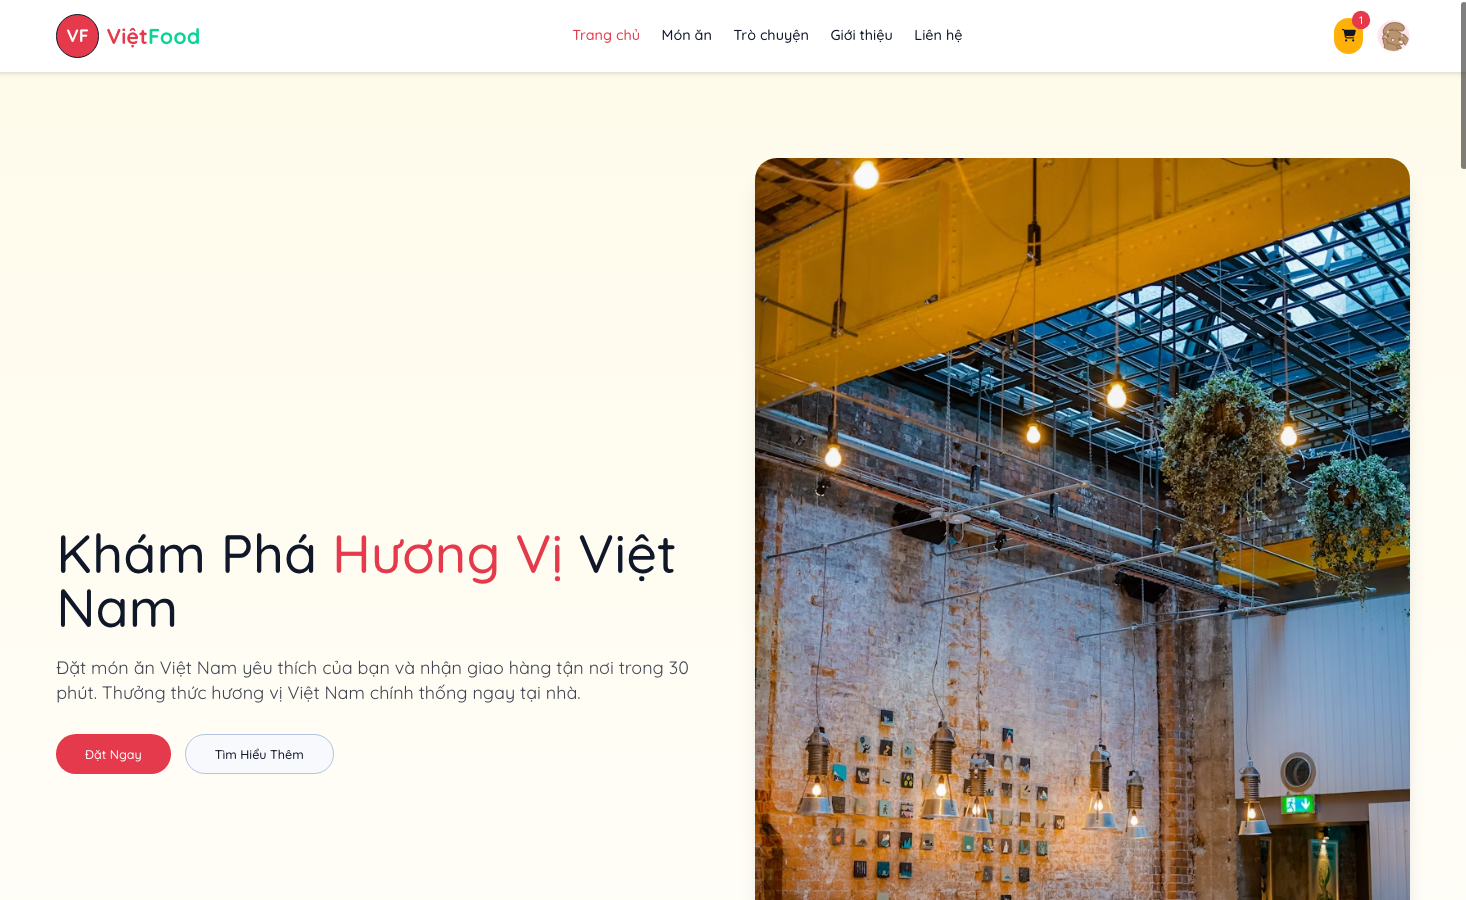
\includegraphics[width=0.9\textwidth]{images/home-page.png}
    \caption{Giao diện trang chủ ứng dụng Việt Food}
    \label{fig:home-page}
\end{figure}

Hình \ref{fig:home-page} thể hiện giao diện chính của ứng dụng, nơi người dùng có thể xem các món ăn nổi bật, tìm kiếm món ăn và dễ dàng đặt hàng.

\begin{figure}[H]
    \centering
    \begin{minipage}{0.48\textwidth}
        \centering
        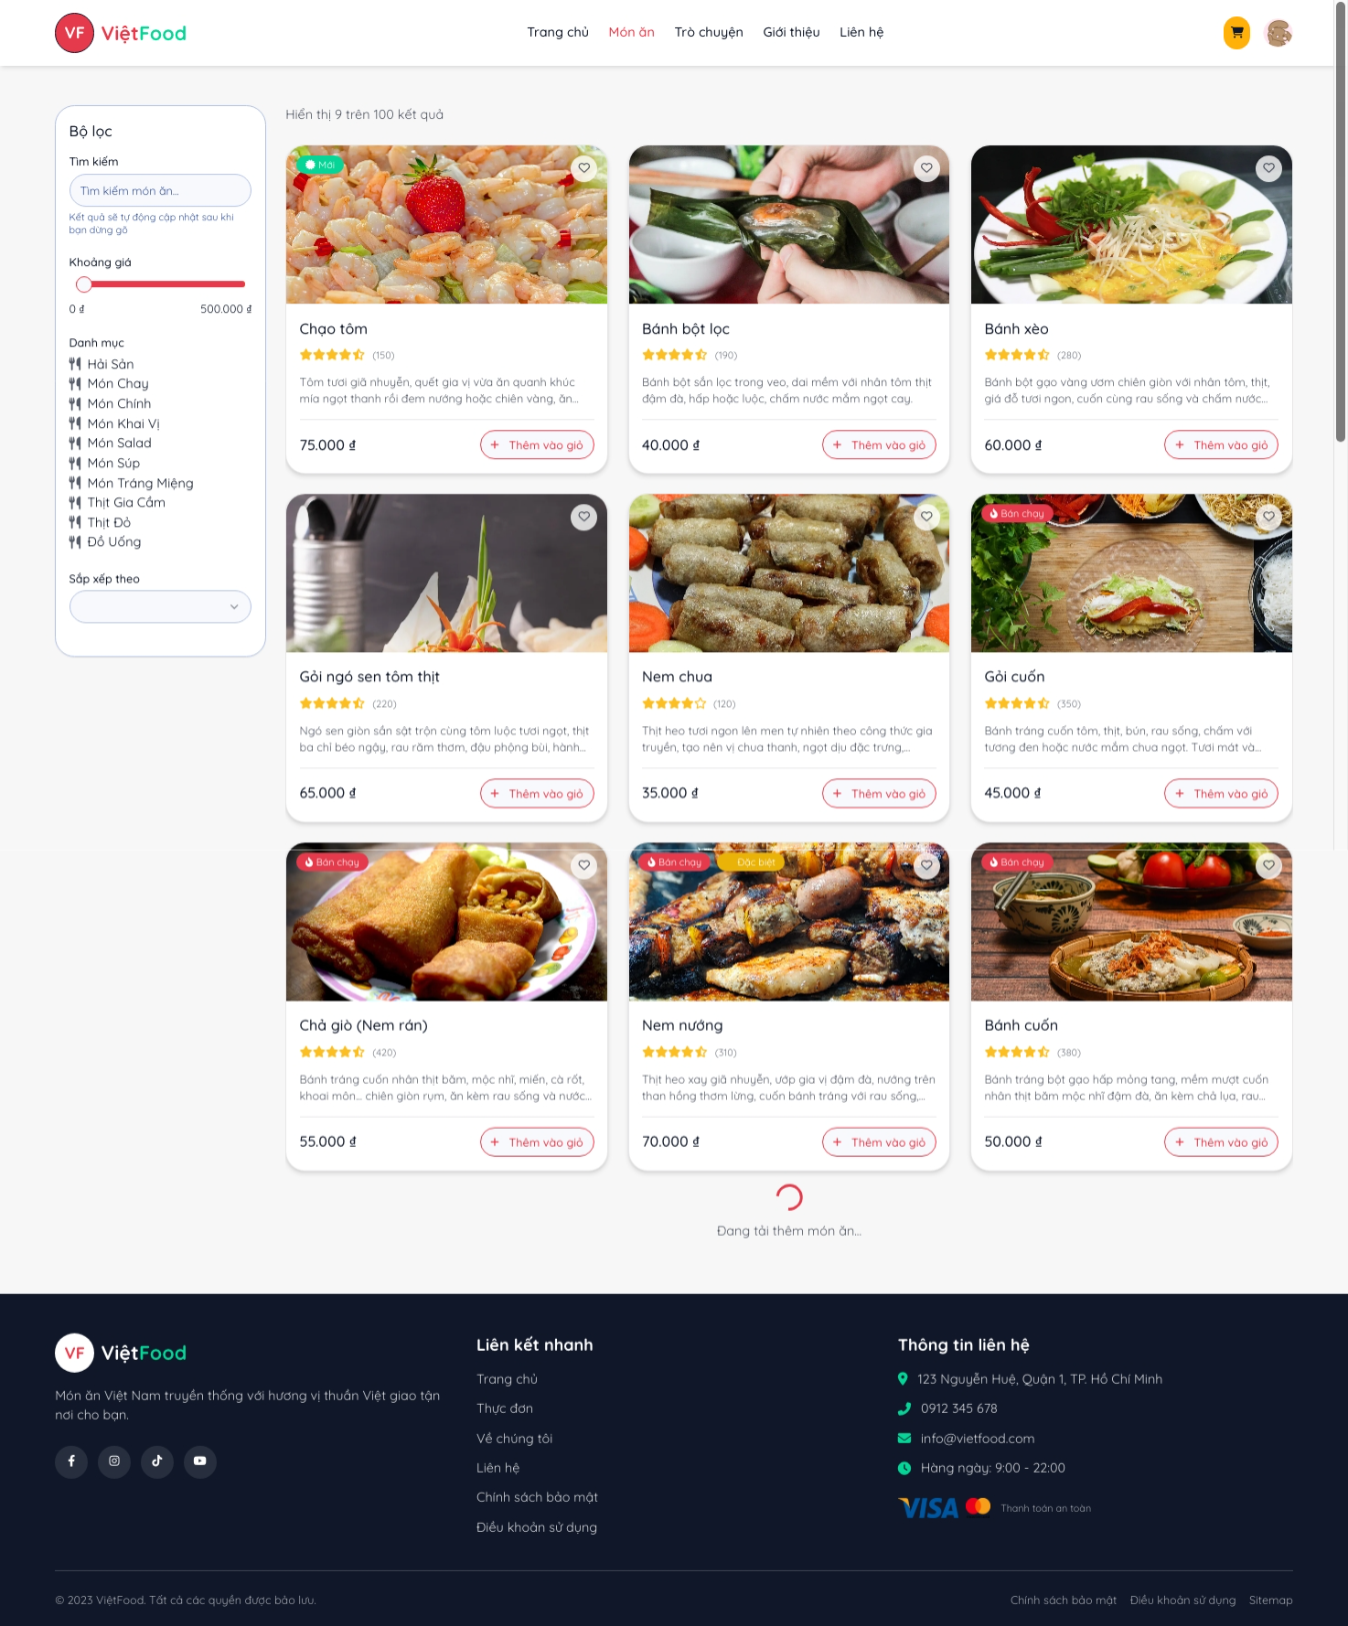
\includegraphics[width=\textwidth]{images/shopping-page.png}
        \caption{Trang đặt món ăn}
        \label{fig:shopping}
    \end{minipage}
    \hfill
    \begin{minipage}{0.48\textwidth}
        \centering
        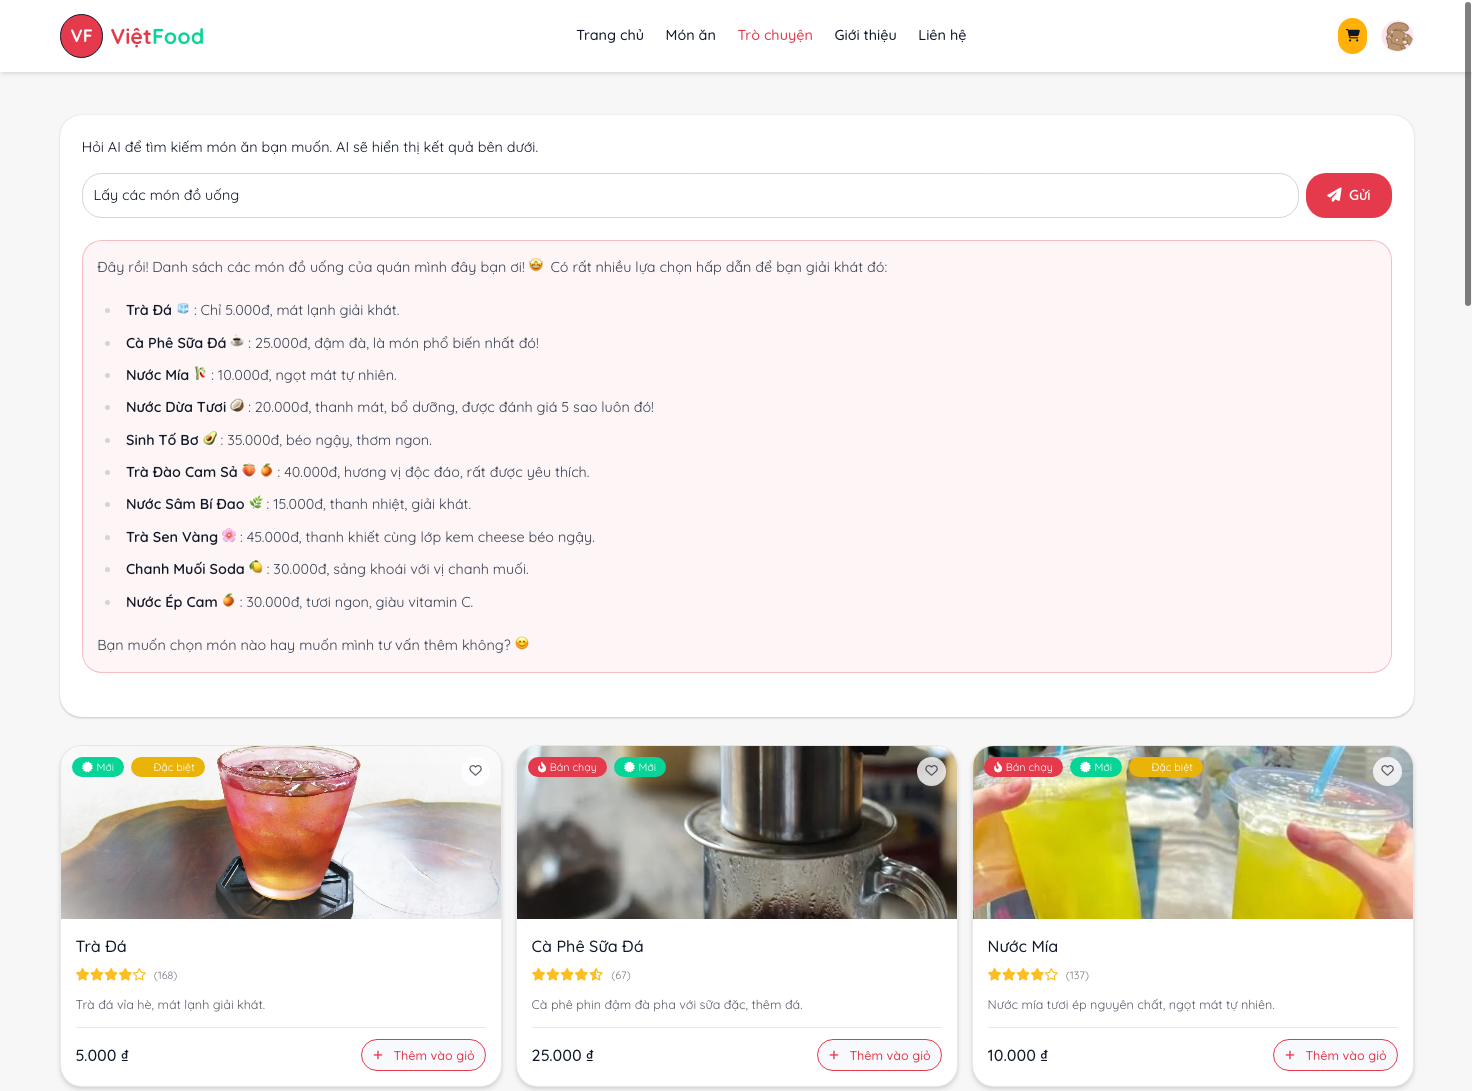
\includegraphics[width=\textwidth]{images/chat-page.png}
        \caption{Tính năng chat hỗ trợ}
        \label{fig:chat}
    \end{minipage}
\end{figure}

\begin{figure}[H]
    \centering
    \begin{minipage}{0.48\textwidth}
        \centering
        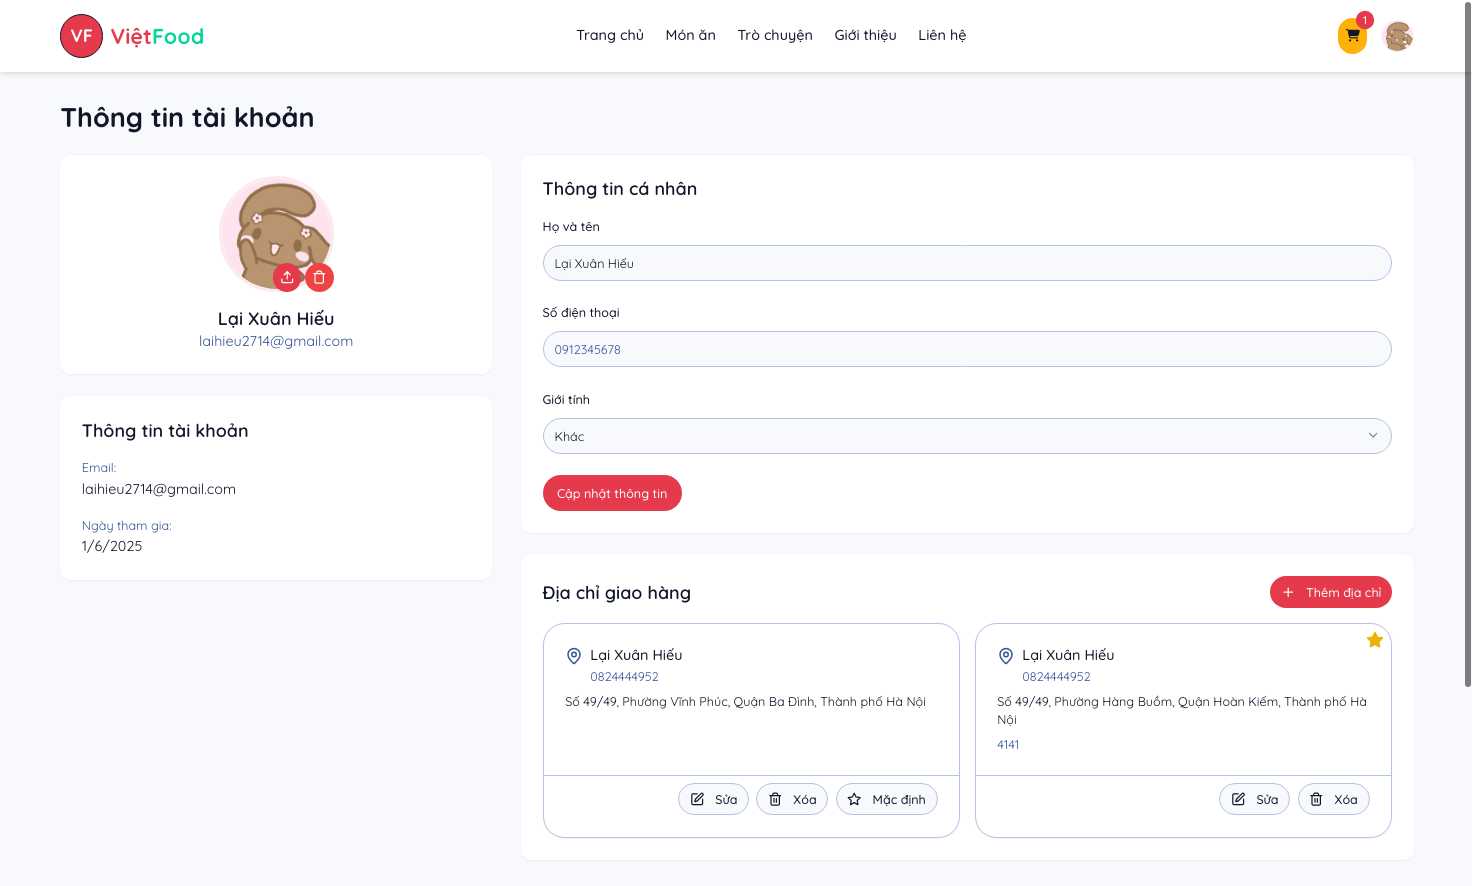
\includegraphics[width=\textwidth]{images/profile-page.png}
        \caption{Trang thông tin cá nhân}
        \label{fig:profile}
    \end{minipage}
    \hfill
    \begin{minipage}{0.48\textwidth}
        \centering
        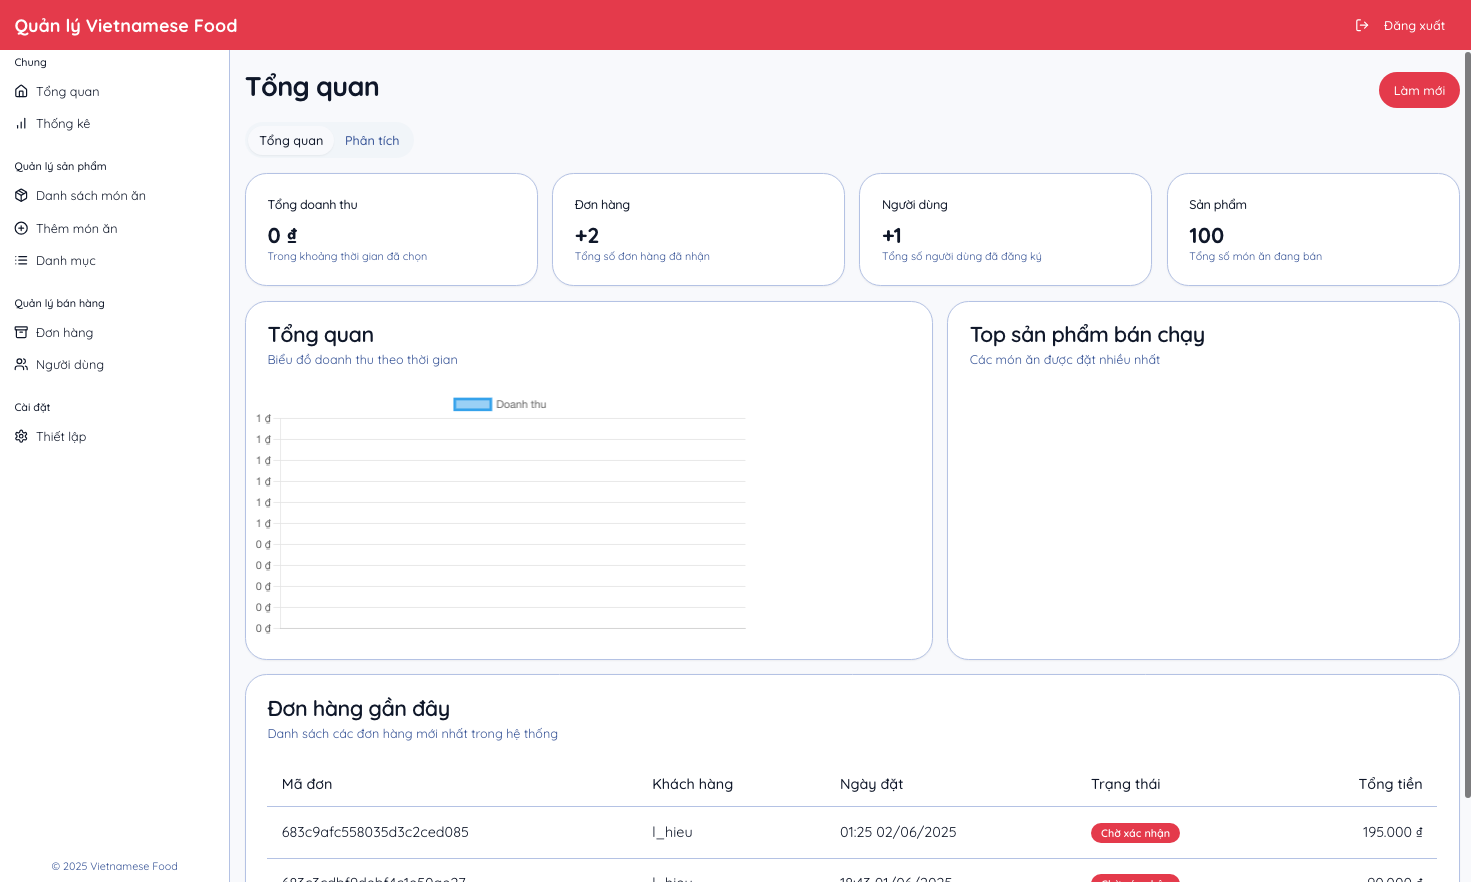
\includegraphics[width=\textwidth]{images/admin-page.png}
        {\footnotesize \caption{Trang quản trị viên}}
        \label{fig:admin}
    \end{minipage}
\end{figure}

\section{Công nghệ sử dụng}
Dự án được xây dựng bằng các công nghệ hiện đại:

\subsection{Backend}
\begin{itemize}
    \item \textbf{Node.js} và \textbf{Express}: Framework cho phát triển ứng dụng web server-side.
    \item \textbf{TypeScript}: Ngôn ngữ lập trình đảm bảo tính mạnh mẽ và an toàn cho mã nguồn.
    \item \textbf{MongoDB}: Cơ sở dữ liệu NoSQL phục vụ lưu trữ dữ liệu phi quan hệ.
    \item \textbf{Redis}: Hệ thống cache bộ nhớ để tối ưu hóa hiệu suất truy vấn.
    \item \textbf{Redis Stream}: Xử lý các tin nhắn và sự kiện real-time.
    \item \textbf{Compression}: Middleware giảm kích thước phản hồi HTTP.
    \item \textbf{Sharp}: Thư viện xử lý và tối ưu hóa hình ảnh.
    \item \textbf{Elasticsearch}: Công cụ tìm kiếm và đánh chỉ mục dữ liệu nhanh chóng.
    \item \textbf{Gemini AI}: Tích hợp trí tuệ nhân tạo cho các tính năng thông minh.
\end{itemize}

\subsection{Frontend}
\begin{itemize}
    \item \textbf{React}: Thư viện JavaScript để xây dựng giao diện người dùng tương tác.
    \item \textbf{TypeScript}: Đảm bảo type safety và khả năng bảo trì cho mã nguồn frontend.
    \item \textbf{Tailwind CSS}: Framework CSS tiện ích giúp phát triển UI nhanh chóng và đồng nhất.
    \item \textbf{React Hook Form}: Quản lý biểu mẫu với hiệu suất cao.
    \item \textbf{Zod}: Thư viện xác thực dữ liệu với TypeScript.
\end{itemize}